\documentclass[a4paper,english]{scrreprt}

% Uncomment to optimize for double-sided printing.
% \KOMAoptions{twoside}

% Set binding correction manually, if known.
% \KOMAoptions{BCOR=2cm}

% Localization options
\usepackage[english]{babel}
\usepackage[T1]{fontenc}
\usepackage[utf8]{inputenc}

% Enhanced verbatim sections. We're mainly interested in
% \verbatiminput though.
\usepackage{verbatim}

% PDF-compatible landscape mode.
% Makes PDF viewers show the page rotated by 90°.
\usepackage{pdflscape}

% Advanced tables
\usepackage{tabu}
\usepackage{longtable}
\usepackage{dcolumn}
\newcolumntype{d}[1]{D{.}{\cdot}{#1} }

% Fancy tablerules
\usepackage{booktabs}

% Graphics
\usepackage{graphicx}

% Current time
\usepackage[useregional=numeric]{datetime2}

% Float barriers.
% Automatically add a FloatBarrier to each \section
\usepackage[section]{placeins}

% Custom header and footer
\usepackage{fancyhdr}

\usepackage{geometry}
\usepackage{layout}

% Math tools
\usepackage{mathtools}
% Math symbols
\usepackage{amsmath,amsfonts,amssymb}
\usepackage{amsthm}

% SI units
\usepackage{siunitx}
\DeclareSIUnit\Molar{\textsc{m}}
\DeclareSIUnit\rpm{\textsc{rpm}}

% Chemistry
\usepackage{mhchem}

% Subfigures & captions
\usepackage{subcaption}
\usepackage{wrapfig}

\DeclarePairedDelimiter\abs{\lvert}{\rvert}

\pagestyle{plain}
% \fancyhf{}
% \lhead{}
% \lfoot{}
% \rfoot{}
% 
% Source code & highlighting
\usepackage{listings}

% Convenience commands
\newcommand{\mailsubject}{2027 - Lab course biochemistry 12}
\newcommand{\maillink}[1]{\href{mailto:#1?subject=\mailsubject}
                               {#1}}

% Should use this command wherever the print date is mentioned.
\newcommand{\printdate}{\today}

\subject{2027 - Lab course biochemistry 1}
\title{12 - Bioinformatics}

\author{Michael Senn \maillink{michael.senn@students.unibe.ch} - 16-126-880 - Group 14}

\date{\printdate}

% Needs to be the last command in the preamble, for one reason or
% another. 
\usepackage{hyperref}


\begin{document}
\maketitle

\chapter{Introduction}

In this experiment we learned how to utilize the various tools and databases
available to us for the purpose of comparing of, and finding information on,
genomes and their encoded proteins. This was done by analyzing the provided
sequenced genome of a repeated cancer patient, looking for mutations which
explain the patient's susceptibility to cancer.

\section{DNA mutations}

There are two types of mutations to DNA, characterizied by whether nucleotides
are modified, or inserted respectively deleted.

\subsection{Point mutations}

Point mutations are mutations where one or multiple nucleotides are changed, eg
a methionine with an arginine. Due to the redundancy of the genetic code, where
multiple three base-pair sequences encode the same amino acid, such a mutation
can be classified as silent - where the new triplet encodes for the same amino
acid, missense - where the new sequence encodes for a different amino acid, and
nonsense - where the new sequence encodes a stop codon.

\subsection{Indel mutations}

Indel mutations are mutations where one or multiple nucleotides are deleted or
inserted. In case of triplets being inserted or deleted they will cause new
amino acids to be added or existing ones to be removed, whereas any other case
will cause a frame-shift, leading to big changes in the amino-acid sequence of
the protein.

\section{Cancer}

Cancer refers to a group of diseases involving uncontrolled growth of cells.
These growths spread within the patient's body, causing a variety of symptoms.
Two categories of genes play an important role in the development of cancer.

Oncogenes are genes which promote cell growth. Mutations which cause new
oncogenes to form, or existing oncogenes to be more heavily expressed by eg
inhibiting regulation mechanisms, can lead to cancer.

Tumor-surpressor genes prevent uncontrolled cell growth by inhibiting cell
division, repairing DNA damage or triggering cell death. Mutations which cause
these genes to become non-functional can also cause cancer.

Cancer is generally caused by multiple mutations, as one mutation will not be
sufficient to cause cancer due to multiple layers of regulation where cell
growth is concerned.

\chapter{Methods}

\section{Extracting sequences of interest from provided sequences}

We were provided with a .SAM file containing the patient's sequenced DNA reads
mapped to the human genome. We utilized a custom Java tool which allowed
specifying the chromosome, strand and basepair ranges of interest, and provided
us with the patient's sequenced nucleotide sequence. The following sequences
were extracted, bp offsets left out for brevity.

\begin{tabu}{lll}
	\toprule
	Gene & Chromosome & Strand \\
	\midrule
	KRAS  & 12 & $-$ \\
	TP53  & 17 & $-$ \\
	BRCA1 & 17 & $-$ \\
	ABL1  & 9  & $+$ \\
	\bottomrule
\end{tabu}

\section{Used tools and databases}

In addition to the custom Java tool mentioned above, the following web-based
tools and databases were used during research.

\begin{itemize}
	\item NCBI Nucleotide BLAST\cite{website:blastn}: Search and alignment of nucleotide sequences in mapped genomes.
	\item ExPASy translate tool\cite{website:expasy}: Translate nucleotide sequences to amino acid sequences.
	\item NCBI Protein BLAST\cite{website:blastp}: Search and alignment of amino acid sequences in protein databases.
	\item UniProt KB\cite{website:uniprot}: Database of known proteins with information on their function, structure, and known mutations.
\end{itemize}

\section{Approach}

The extracted nucleotide sequences were BLAST-ed to find matches in the human
genome. Mutations were written down. Afterwards the patient's nucleotide
sequence was translated into a sequence of amino acids, and those once more
BLAST-ed to find matching human proteins, with mutations being written down.
Lastly, the function and effect of so found mutations was researched.

\chapter{Results}
% For all: Functions, relation of mutation to cancer

\section{KRAS}

KRAS is an oncogene. In its active form it promotes cell-growth, in its
inactive it does not.

\subsection{Observed mutations}

With KRAS, a 227 G>T missense mutation can be observed in the genome, as seen
in figure \ref{fig:kras_mut_dna}. This leads to a G12V mutation in the protein,
as seen in figure \ref{fig:kras_mut_prot}.

This mutation is a known variant of KRAS (VAR\_006840), known to be linked to
various types of cancer.\cite{website:uniprot_kras}

\begin{figure}
	\centering
	\begin{subfigure}{.95\textwidth}
		\centering
		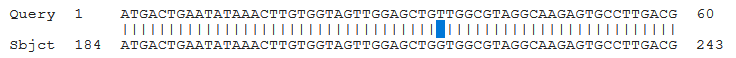
\includegraphics[width=\linewidth]{img/kras_mut_dna.png}
		\caption{Mutation in KRAS DNA}
		\label{fig:kras_mut_dna}
	\end{subfigure}%
	\vskip\baselineskip
	\begin{subfigure}{.95\textwidth}
		\centering
		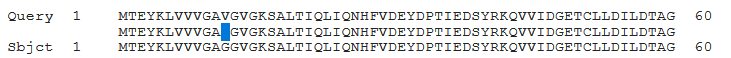
\includegraphics[width=\linewidth]{img/kras_mut_prot.png}
		\caption{Mutation in KRAS Protein}
		\label{fig:kras_mut_prot}
	\end{subfigure}%
	\caption{Mutations of KRAS}
	\label{fig:kras_mut}
\end{figure}

\subsection{Effect on interaction with proteins and protein function}

The mutation lies within one of the binding sites for GTP used for regulation
of protein inactivity. As such it might cause regulating proteins to be unable
to bind.  This may cause the protein to be permanently active, promoting
uncontrolled cell-growth.\cite{website:uniprot_kras}

\section{TP53}

TP53 is a tumor-surpressor which works by inhibiting cell growth, or triggering
cell death, in presence of damaged DNA.\cite{website:uniprot_tp53}

\subsection{Observed mutations}

With TP53, a deletion of nucleotides 875 through 1195 can be observed in figure
\ref{fig:tp53_mut_dna}. This leads to amino acids 225 through 331 missing in
the translated protein as seen in figure \ref{fig:kras_mut_prot}. The mutation
is located within exons 9, 10 and 11.

\begin{figure}
	\centering
	\begin{subfigure}{.95\textwidth}
		\centering
		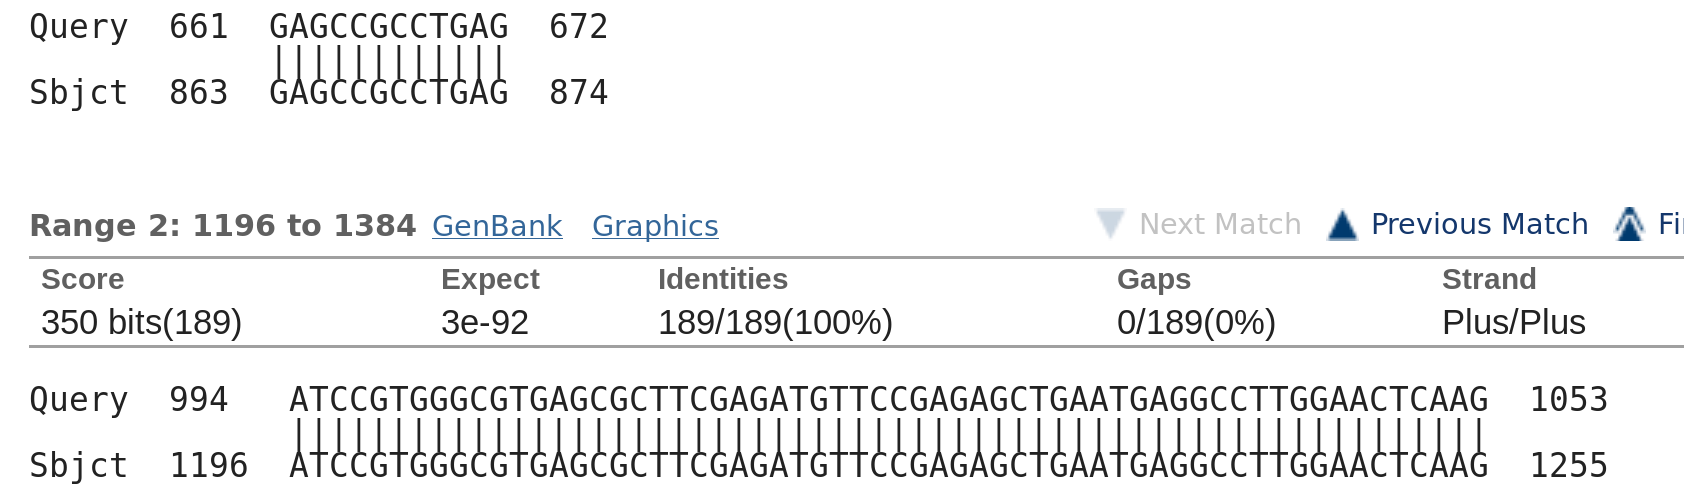
\includegraphics[width=\linewidth]{img/tp53_mut_dna.png}
		\caption{Mutation in TP53 DNA}
		\label{fig:tp53_mut_dna}
	\end{subfigure}%
	\vskip\baselineskip
	\begin{subfigure}{.95\textwidth}
		\centering
		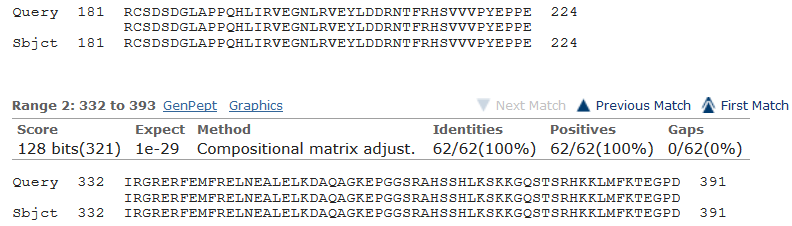
\includegraphics[width=\linewidth]{img/tp53_mut_prot.png}
		\caption{Mutation in TP53 Protein}
		\label{fig:tp53_mut_prot}
	\end{subfigure}%
	\caption{Mutations of TP53}
	\label{fig:tp53_mut}
\end{figure}

\subsection{Effect on potein function}

TP53 has binding units able to accept \ce{Zn^{2+}} in four locations, which are of
importance for proper conformation.\cite{website:uniprot_tp53} Two of these
binding sites, at positions 238 and 242 respectively, are lost because of the
mutation. Furthermore the mutation leads to the loss of a big part of a subunit
responsible for binding to DNA shown in figure \ref{fig:tp53_subunits}.

\begin{figure}
	\centering
	\includegraphics[width=\linewidth]{img/tp53_subunits.png}
	\caption{TP53 subunits\cite{wiki:tp53_subunits}}
	\label{fig:tp53_subunits}
\end{figure}

Such a mutation will likely prevent the protein from folding properly, as well
as prevent it from binding to and recognizing damaged DNA. This may very well
explain the patient's susceptibility to cancer, as cells with mutated DNA will
be able to replicate freely, since TP53 is unable to induce cell death.

\subsection{PCR results}

The results of the PRC shown in figure \ref{fig:tp53_pcr} show as expected the
4000 bp long nucleotide sequence in the mother's genome. In the daughter's
cancerous tissue only a nucleotide sequence of roughly 1000 bp is visible,
indicating that parts of the missing area lies between the forward and reverse
primer.

Furthermore even healthy skin cells of the daughter contain partially mutated
DNA, indicating that one of the two alleles of the daughter's skin cells has
mutated.

\begin{figure}
	\centering
	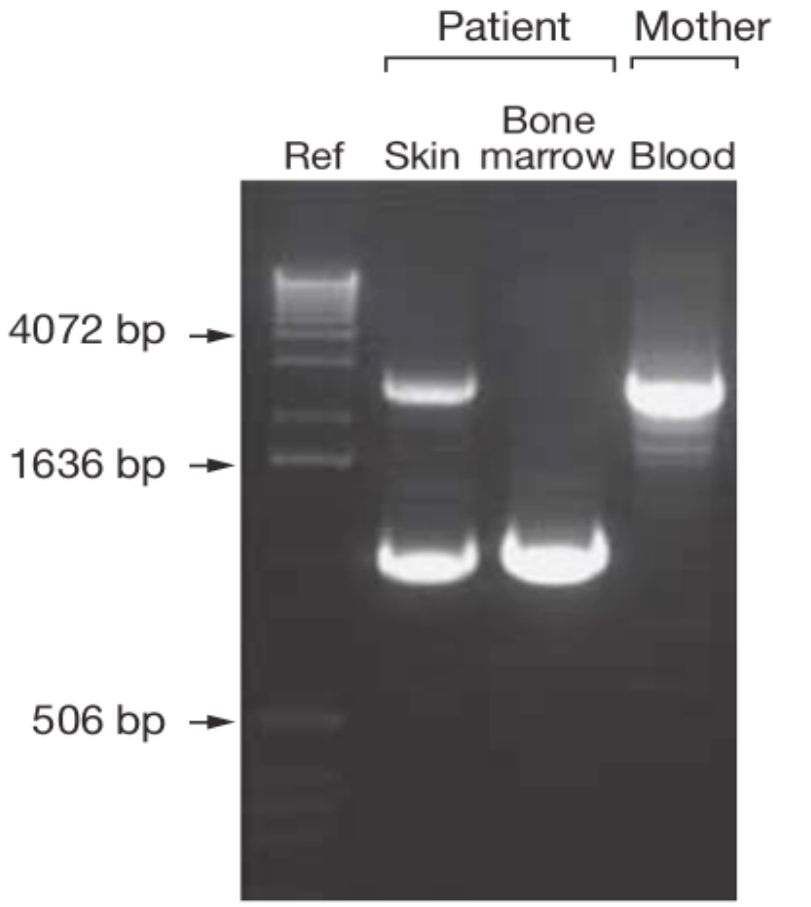
\includegraphics[width=0.5\linewidth]{img/tp53_pcr.png}
	\caption{TP53 PCR results}
	\label{fig:tp53_pcr}
\end{figure}

\section{BRCA1}

BRCA1 is a tumor-surpressor which plays an important role in repairing damaged
DNA by repairing double-stranded DNA breaks.

\subsection{Observed mutations}

Within the sequence of BRCA1 a 5565 T>G missense mutation can be observed as
shown in figure \ref{fig:brca1_mut_dna}. This leads to a M 1775 R substitution
within the protein as seen in figure \ref{fig:brca1_mut_prot}.

\begin{figure}
	\centering
	\begin{subfigure}{.95\textwidth}
		\centering
		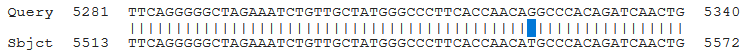
\includegraphics[width=\linewidth]{img/brca1_mut_dna.png}
		\caption{Mutation in BRCA1 DNA}
		\label{fig:brca1_mut_dna}
	\end{subfigure}%
	\vskip\baselineskip
	\begin{subfigure}{.95\textwidth}
		\centering
		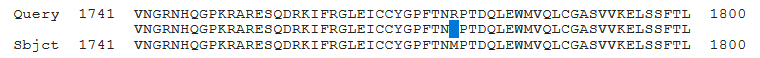
\includegraphics[width=\linewidth]{img/brca1_mut_prot.png}
		\caption{Mutation in BRCA1 Protein}
		\label{fig:brca1_mut_prot}
	\end{subfigure}%
	\caption{Mutations of BRCA1}
	\label{fig:brca1_mut}
\end{figure}

\subsection{Effects on chemical properties of protein}

The exchange of methionine with arginine causes the replacement of a
medium-sized hydrophobic amino acid to a large-sized basic
one.\cite{website:expasy_brca1} A very notable change is the difference in the
charge distribution of the protein, one example of which is shown in figure
\ref{fig:brca1_charge_distribution}.

\begin{figure}
	\centering
	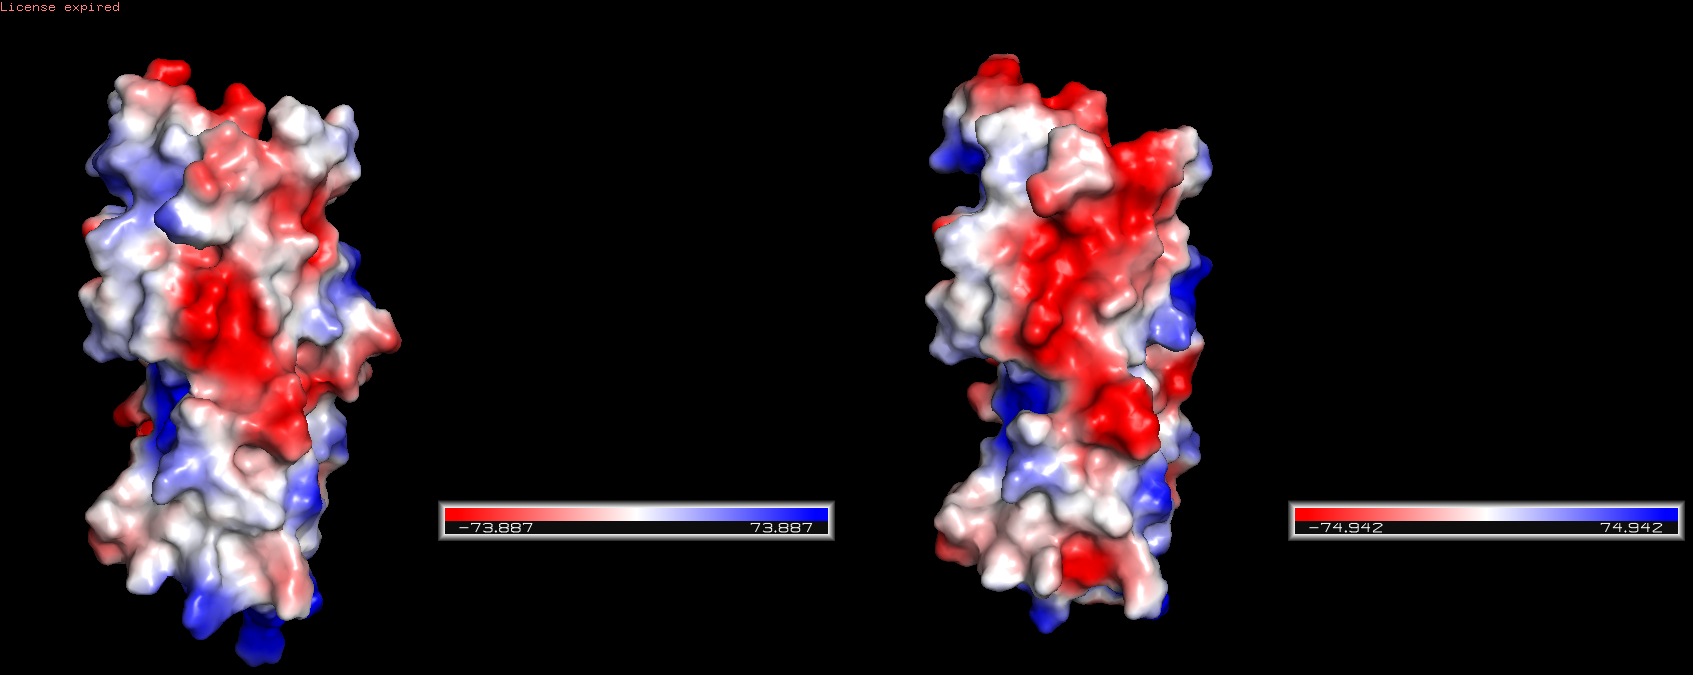
\includegraphics[width=\linewidth]{img/brca1_charge_distribution.png}
	\caption{Charge distribution of wild-type (right) vs mutated (left) BRCA1}
	\label{fig:brca1_charge_distribution}
\end{figure}

\subsection{Effect on protein function}

The M 1775 R mutation is a known variant, which will influence protein
stability and prevent interaction with BRIP1 and
RBBP8.\cite{website:uniprot_brca1} Both the BRCA1/BRIP1 as well as the
BRCA1/RBBP8 complex play a role in BRCA1's ability to repair damaged DNA. As
such, inability to interact with these may hinder its tumor-surpressant
function.

\section{ABL1}

ABL1 is a proto-oncogene, playing a role in many processes of cell
growth.\cite{website:uniprot_abl1} In its active form it promotes cell growth
while in its inactive form it does not. The change between active and inactive
form involves a change of conformation, as well as an $\alpha$ helix near
Glu-286.\cite{skriptv12}

\subsection{Observed mutations}

The patient's ABL1 gene has three groups of mutations. One insert and one
delete causing a frameshift in a small region, and an additional missense
mutation within.

As shown in figure \ref{fig:abl1_mut_dna}, there is an additional C between
nucleotides 1022 and 1023. In addition there is a 1043 T>C mutation, and a
deletion of the A at position 1082.  This causes 19 substitutions in the
protein, of which four are conservative.  Details are found in figure
\ref{fig:abl1_mut_prot}. Glu 286 suffers a E286R mutation.

\begin{figure}
	\centering
	\begin{subfigure}{.95\textwidth}
		\centering
		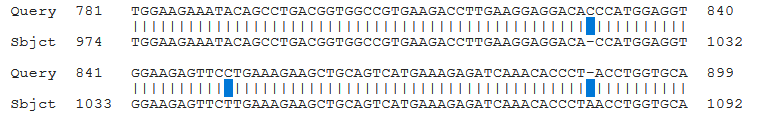
\includegraphics[width=\linewidth]{img/abl1_mut_dna.png}
		\caption{Mutation in ABL1 DNA}
		\label{fig:abl1_mut_dna}
	\end{subfigure}%
	\vskip\baselineskip
	\begin{subfigure}{.95\textwidth}
		\centering
		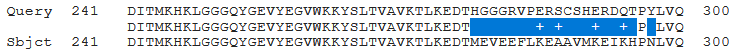
\includegraphics[width=\linewidth]{img/abl1_mut_prot.png}
		\caption{Mutation in ABL1 Protein}
		\label{fig:abl1_mut_prot}
	\end{subfigure}%
	\caption{Mutations of ABL1}
	\label{fig:abl1_mut}
\end{figure}

\subsection{Effect on secondary structure}

\begin{figure}
	\centering
	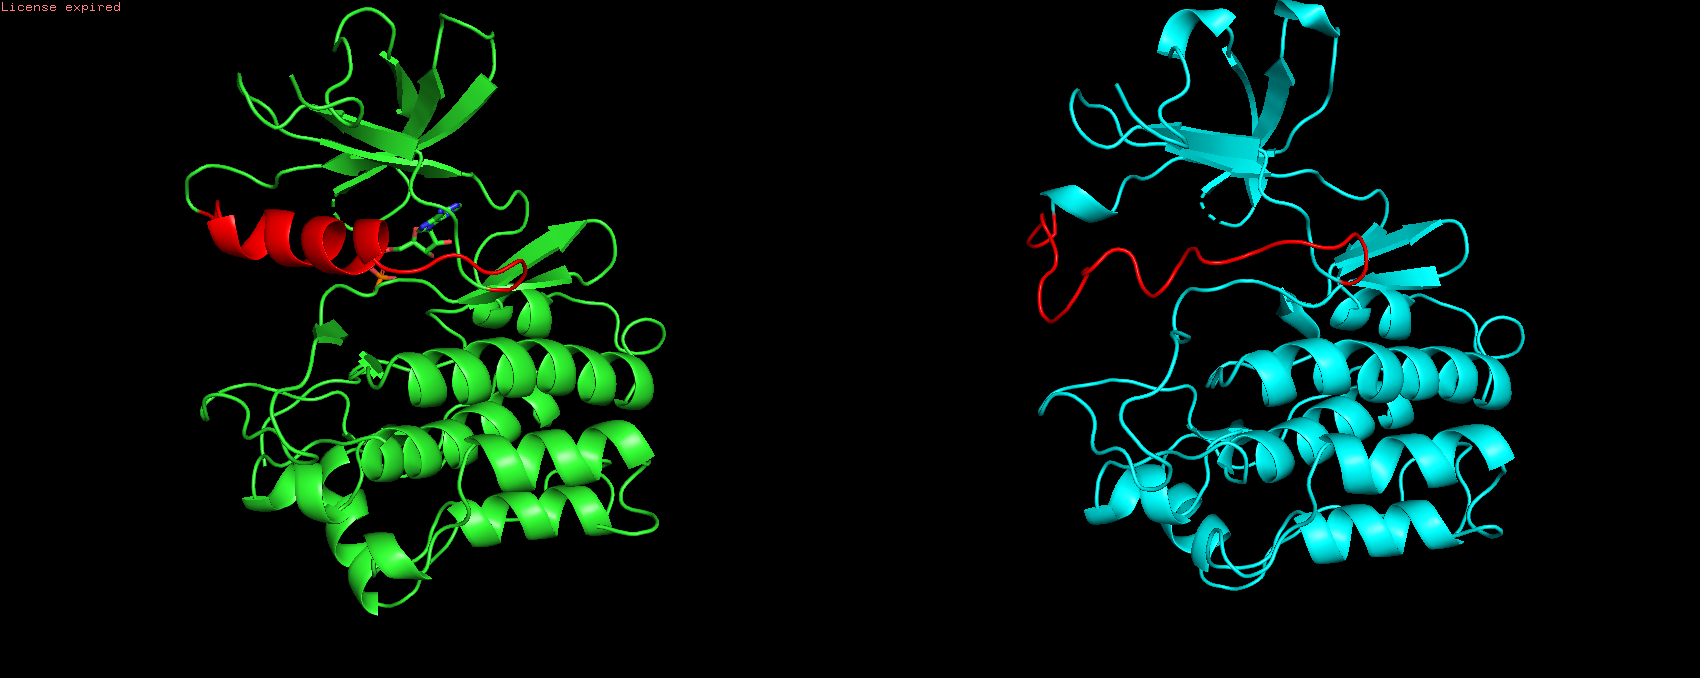
\includegraphics[width=\linewidth]{img/abl1_structure.png}
	\caption{Structure of wild-type vs mutated ABL1. Wild-type on left in green}
	\label{fig:abl1_structure}
\end{figure}

As is visible in figure \ref{fig:abl1_structure}, the substitutions lead to
loss of an $\alpha$ helix near Glu-286. There are other less-pronounced changes
in the secondary structure, such as to the anti-parallel $\beta$-sheet right
above the lost $\alpha$ helix.

\subsection{Effect on protein function}

Due to the effect of the lost $\alpha$-helix on regulation of the
protein\cite{skriptv12}, it is likely that its loss leads to the protein being
stuck in a permanently active state, promoting uncontrolled cell growth and
therefore cancer.


\bibliographystyle{vancouver}
\bibliography{references}

\end{document}
